\documentclass[tikz,border=3mm]{standalone}
\usepackage{amsmath,amssymb}
\renewcommand{\familydefault}{\sfdefault}
\usepackage{tikz}
\usepackage{pgfplots}
\pgfplotsset{compat=1.18}
\usetikzlibrary{
  arrows.meta,
  positioning,
  calc,
  fit,
  backgrounds,
  shapes.geometric,
  pgfplots.fillbetween
}

\definecolor{R7Navy}{HTML}{17324D}
\definecolor{R7Teal}{HTML}{0A8F8F}
\definecolor{R7Gold}{HTML}{E0A12B}
\definecolor{R7Coral}{HTML}{D85D55}
\definecolor{R7Violet}{HTML}{6757C7}
\definecolor{R7Sky}{HTML}{5AA6C8}
\definecolor{R7Ink}{HTML}{243746}
\definecolor{R7Muted}{HTML}{667784}
\definecolor{R7Pale}{HTML}{EEF4F5}
\definecolor{R7Warm}{HTML}{FFF6E5}
\definecolor{R7Paper}{HTML}{FCFDFD}

\tikzset{
  r7box/.style={
    rounded corners=2.2mm,
    very thick,
    align=center,
    minimum height=23mm,
    text width=29mm,
    inner sep=3.2mm
  },
  r7arrow/.style={
    -{Stealth[length=2.4mm,width=1.8mm]},
    line width=1.0pt,
    color=R7Muted
  },
  r7tag/.style={
    font=\bfseries\scriptsize,
    text=R7Navy,
    fill=white,
    inner sep=1.2pt
  }
}

\pgfplotsset{
  r7axis/.style={
    axis line style={R7Ink, line width=0.8pt},
    tick style={R7Ink, line width=0.7pt},
    tick label style={font=\footnotesize, text=R7Ink},
    label style={font=\small, text=R7Ink},
    title style={font=\bfseries\small, text=R7Navy, yshift=1mm},
    grid=both,
    major grid style={draw=R7Muted!22, line width=0.45pt},
    minor grid style={draw=R7Muted!10, line width=0.35pt},
    legend style={
      draw=none,
      fill=white,
      fill opacity=0.92,
      text opacity=1,
      font=\scriptsize,
      cells={anchor=west}
    }
  }
}

\begin{document}
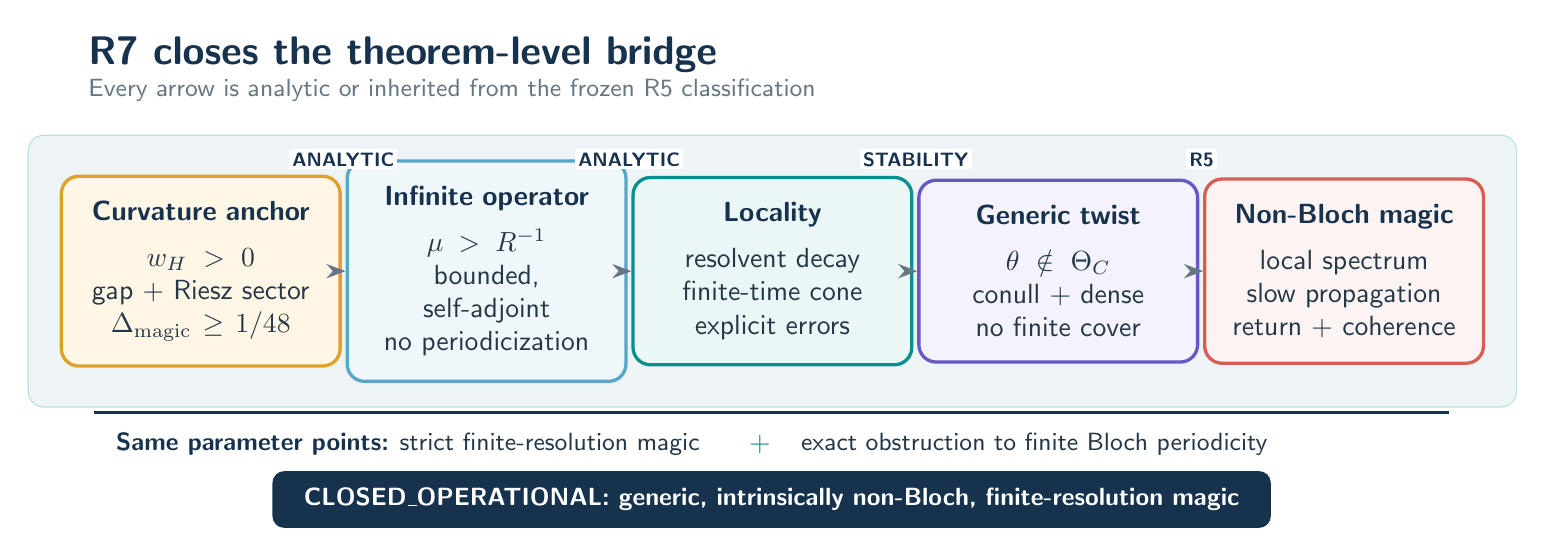
\begin{tikzpicture}[font=\sffamily]
  \node[anchor=west,font=\bfseries\Large,text=R7Navy] at (0,4.0)
    {R7 closes the theorem-level bridge};
  \node[anchor=west,font=\small,text=R7Muted] at (0,3.55)
    {Every arrow is analytic or inherited from the frozen R5 classification};

  \node[r7box,draw=R7Gold,fill=R7Warm,text=R7Ink] (anchor) at (1.55,1.25) {
    \textbf{\color{R7Navy}Curvature anchor}\\[1.6mm]
    $w_H>0$\\
    gap + Riesz sector\\
    $\Delta_{\rm magic}\ge 1/48$
  };
  \node[r7box,draw=R7Sky,fill=R7Sky!9,text=R7Ink] (operator) at (5.18,1.25) {
    \textbf{\color{R7Navy}Infinite operator}\\[1.6mm]
    $\mu>R^{-1}$\\
    bounded, self-adjoint\\
    no periodicization
  };
  \node[r7box,draw=R7Teal,fill=R7Teal!8,text=R7Ink] (locality) at (8.81,1.25) {
    \textbf{\color{R7Navy}Locality}\\[1.6mm]
    resolvent decay\\
    finite-time cone\\
    explicit errors
  };
  \node[r7box,draw=R7Violet,fill=R7Violet!7,text=R7Ink] (generic) at (12.44,1.25) {
    \textbf{\color{R7Navy}Generic twist}\\[1.6mm]
    $\theta\notin\Theta_C$\\
    conull + dense\\
    no finite cover
  };
  \node[r7box,draw=R7Coral,fill=R7Coral!7,text=R7Ink] (magic) at (16.07,1.25) {
    \textbf{\color{R7Navy}Non-Bloch magic}\\[1.6mm]
    local spectrum\\
    slow propagation\\
    return + coherence
  };

  \draw[r7arrow] (anchor) -- (operator);
  \draw[r7arrow] (operator) -- (locality);
  \draw[r7arrow] (locality) -- (generic);
  \draw[r7arrow] (generic) -- (magic);
  \node[r7tag] at (3.36,2.67) {ANALYTIC};
  \node[r7tag] at (6.99,2.67) {ANALYTIC};
  \node[r7tag] at (10.63,2.67) {STABILITY};
  \node[r7tag] at (14.26,2.67) {R5};

  \begin{scope}[on background layer]
    \node[rounded corners=2mm,fill=R7Pale,draw=R7Teal!28,
      fit=(anchor)(magic),inner xsep=4mm,inner ysep=5mm] {};
  \end{scope}

  \draw[line width=1.1pt,R7Navy]
    (0.2,-0.55) -- (17.4,-0.55);
  \node[anchor=west,font=\bfseries\small,text=R7Navy] at (0.35,-0.95)
    {Same parameter points:};
  \node[anchor=west,font=\small,text=R7Ink] at (3.95,-0.95)
    {strict finite-resolution magic};
  \node[font=\bfseries,text=R7Teal] at (8.65,-0.95) {$+$};
  \node[anchor=west,font=\small,text=R7Ink] at (9.05,-0.95)
    {exact obstruction to finite Bloch periodicity};

  \node[rounded corners=1.5mm,fill=R7Navy,text=white,
    font=\bfseries\small,inner xsep=4mm,inner ysep=2.2mm]
    at (8.8,-1.65)
    {CLOSED\_OPERATIONAL: generic, intrinsically non-Bloch, finite-resolution magic};
\end{tikzpicture}
\end{document}
